\documentclass[main.tex,fontsize=8pt,paper=a4,paper=portrait,DIV=calc,]{scrartcl}
% Document
\usepackage[T1]{fontenc}
\usepackage[dvipsnames]{xcolor}
\usepackage[nswissgerman,english]{babel}
\renewcommand{\familydefault}{\sfdefault}

% Format
\usepackage[top=5mm,bottom=1mm,left=5mm,right=5mm]{geometry}
%\setlength{\headheight}{\baselineskip}
%\setlength{\headsep}{0mm}

%\usepackage{scrlayer-scrpage}
%\clearpairofpagestyles
%\chead{{\bfseries\TITLE, \AUTHOR, \pagename~\thepage}}

%\addtokomafont{pagehead}{\upshape}

\usepackage{multicol}
\setlength{\columnsep}{2mm}
\setlength{\columnseprule}{0.1pt}

% Math
\usepackage{amsmath}
\usepackage{amssymb}
\usepackage{amsfonts}

% Code
\usepackage{fancyvrb, etoolbox, listings, xcolor}
%\usemintedstyle{bw}

%\newminted[shell]{bash}{
%fontsize=\footnotesize,
%fontfamily=tt,
%breaklines=true,
%frame=single,
%framerule=0.1pt,
%framesep=2mm,
%tabsize=2
%}
%\newminted{css}{
%breaklines=true,
%tabsize=4,
%autogobble=true,
%escapeinside=||,
%stripall=true,
%stripnl=true,
%}

    \definecolor{lightgray}{rgb}{0.95, 0.95, 0.95}
    \definecolor{darkgray}{rgb}{0.4, 0.4, 0.4}
    \definecolor{purple}{rgb}{0.65, 0.12, 0.82}
    \definecolor{ocherCode}{rgb}{1, 0.5, 0} % #FF7F00 -> rgb(239, 169, 0)
    \definecolor{blueCode}{rgb}{0, 0, 0.93} % #0000EE -> rgb(0, 0, 238)
    \definecolor{greenCode}{rgb}{0, 0.6, 0} % #009900 -> rgb(0, 153, 0)
    \definecolor{teal}{rgb}{0.0, 0.5, 0.5}

\lstdefinestyle{code}{
    identifierstyle=\color{black},
    keywordstyle=\color{blue}\bfseries\small,
    ndkeywordstyle=\color{greenCode}\bfseries\small,
    stringstyle=\color{ocherCode}\ttfamily\small,
    commentstyle=\color{teal}\ttfamily\textit\small,
    basicstyle=\ttfamily\small,
    breakatwhitespace=false,         
    breaklines=true,                 
    captionpos=b,                    
    keepspaces=true,                 
    showspaces=false,                
    showstringspaces=false,
    showtabs=false,                  
    tabsize=2,
    belowskip=-5pt
}



% Images
\usepackage{graphicx}
\newcommand{\pic}{\includegraphics[scale=0.3]}
\graphicspath{{Screenshots/}{../Screenshots}}
\makeatletter
\def\pictext#1#2{%
    \@ifnextchar[{%
    \pictext@iiiii{#1}{#2}%
    }{%
      \pictext@iiiii{#1}{#2}[0.5,0.4,0.3]% Default is 5
    }%
}
\def\pictext@iiiii#1#2[#3,#4,#5]{\begin{minipage}{#3\textwidth}\includegraphics[scale=#4]{#1}\end{minipage}\begin{minipage}{#5\textwidth}#2\end{minipage}}
\def\minipg#1#2{%
    \@ifnextchar[{%
    \minipg@iiii{#1}{#2}%
    }{%
      \minipg@iiii{#1}{#2}[0.3,0.6]% Default is 5
    }%
}
\def\minipg@iiii#1#2[#3,#4]{\vspace{0.8mm}\begin{minipage}{#3\textwidth}#1\end{minipage}\begin{minipage}{#4\textwidth}#2\end{minipage}{\vspace{0.8mm}}}
\makeatother

%\newenvironment{minty}[2]% environment name
%{% begin code
%  \begin{minipage}{#1}
%  \begin{minted}{#2}
%}%
%{% end code
%  \end{minted}
%  \end{minipage}
%  \end{minty}\ignorespacesafterend
%} 

% Smaller Lists
\usepackage{enumitem}
\setlist[itemize,enumerate]{leftmargin=3mm, labelindent=0mm, labelwidth=1mm, labelsep=1mm, nosep}
\setlist[description]{leftmargin=0mm, nosep}
\setlength{\parindent}{0cm}

% Smaller Titles
\usepackage[explicit]{titlesec}

%% Color Boxes
\newcommand{\sectioncolor}[1]{\colorbox{black!60}{\parbox{0.989\linewidth}{\color{white}#1}}}
\newcommand{\subsectioncolor}[1]{\colorbox{black!50}{\parbox{0.989\linewidth}{\color{white}#1}}}
\newcommand{\subsubsectioncolor}[1]{\colorbox{black!40}{\parbox{0.989\linewidth}{\color{white}#1}}}
\newcommand{\paragraphcolor}[1]{\colorbox{black!30}{\parbox{0.989\linewidth}{\color{white}#1}}}
\newcommand{\subparagraphcolor}[1]{\colorbox{black!20}{\parbox{0.989\linewidth}{\color{white}#1}}}

%% Title Format
\titleformat{\section}{\vspace{0.5mm}\bfseries}{}{0mm}{\sectioncolor{\thesection~#1}}[{\vspace{0.5mm}}]
\titleformat{\subsection}{\vspace{0.5mm}\bfseries}{}{0mm}{\subsectioncolor{\thesubsection~#1}}[{\vspace{0.5mm}}]
\titleformat{\subsubsection}{\vspace{0.5mm}\bfseries}{}{0mm}{\subsubsectioncolor{\thesubsubsection~#1}}[{\vspace{0.5mm}}]
\titleformat{\paragraph}{\vspace{0.5mm}\bfseries}{}{0mm}{\paragraphcolor{\theparagraph~#1}}[{\vspace{0.5mm}}]
\titleformat{\subparagraph}{\vspace{0.5mm}\bfseries}{}{0mm}{\subparagraphcolor{\thesubparagraph~#1}}[{\vspace{0.5mm}}]

%% Title Spacing
\titlespacing{\section}{0mm}{0mm}{0mm}
\titlespacing{\subsection}{0mm}{0mm}{0mm}
\titlespacing{\subsubsection}{0mm}{0mm}{0mm}
\titlespacing{\paragraph}{0mm}{0mm}{0mm}
\titlespacing{\subparagraph}{0mm}{0mm}{0mm}

%% format cells
\usepackage[document]{ragged2e}
\usepackage{array, makecell}
\renewcommand{\arraystretch}{2}
\newcommand{\mc}{\makecell[{{m{1\linewidth}}}]}


\begin{document}
\begin{table}[h!]
\section{Terms and Definitions}
\begin{tabular}{|m{0.2\linewidth}|m{0.755\linewidth}|}
\hline
AGI Articifial General Intelligence & This is the hypothetical goal of achieving an AI that can perform general task as good or even better than a human. Aka, the goal is to essentially mimic a human in their general life. \\
\hline
Turing test & This is an idea that if a machine can do X task just like a human, aka indistinguishable from the human, then the machine has passed the Turing test. The problem with this however, is that a machine needs to learn to lie, since a human can do this as well -> see the pinoccio problem. The second problem is that certain tasks are too complex for humans but might not be for a machine, in this case the Turing test simply makes no sense. \\
\hline
Machine Learning & Machine Learning is comprised of 3 different techniques. Supervised learning, unsupervised learning and reinforcement learning. Supervised and unsupervised are not that different other tan the presence of the human. Reinforcement learning however is different as the AI is rewarded for "good" behavior/results and "punished" for bad behavior/results. \\
\hline
NLP Natural Language Processing & The research field of trying to achieve both understanding and creation of natural human language by AI. While development has been in the works for quite a while, because AI can't understand context, it is still very much "in beta". \\
\hline
\emph{The 4 Ingredients of Machine-Learning} & 
\vspace{2mm}
\begin{enumerate}
\item Data \newline
In order for a machine to learn anything you need to provide it with data to work with.
\item Cost-Function(Loss) \newline
You need a way to tell your machine what is considered to be good or bad. \newline
Without it the machine can't learn from it's previous endeavors.\newline
\item Model \newline
This can be something simple as 2 parameters like \(y_i = ax_i + b\) or something complicated like a neural network.\newline
We usually use something like \emph{tensorflow} or \emph{pytorch} to define the model\newline
At the end of the day it is always some sort of \textbf{mathematical function!}
\item Optimization
An algorithm that minimizes the amount of parameters needed for the cost function. \newline
Usually something like Stochastic Gradient Descent(SGD), ADAM, RMSProp 
\end{enumerate}
\vspace{2mm}
There are many more, but these 4 are the most important. You might also care about performance optimization\newline
visualization and validation though.\\
\hline
\end{tabular}
\subsection{Representation of words}
\begin{tabular}{|m{0.2\linewidth}|m{0.755\linewidth}|}
\hline
\textbf{\emph{One-hot vector}} & \minipg{ 
This is a vector with 1 value set to 1, this represents the word.\newline
If you now iterate over a sentence, you will end up with a matrix.\newline}
{\pic{2022-09-29:08:51:08.png}}[0.3,0.7]\newline
Problems with this approach\newline
\begin{itemize}
\item high dimensionality\newline
for 100,000 words you would need 100,000 dimensions to the vector.\newline
\item sparse information\newline
The vast majority of the vector aka all but one, is just 0's, this is not data!.\newline
\item no generalization \newline
There is no context for words, no groups, no terms.\newline
For example a car is associated with tires but not with mangos.\newline
This method can't associate anything with anything.\newline
\end{itemize}
\\
\hline
\textbf{\emph{Indexing}} & 
Indexing simply assigns a number to a word. \newline
This approach solves the problem of having a vector with mostly 0's,\newline
but it does not solve the problem of not having context, a mango still has no boundary.\\
\hline
\textbf{\emph{Distributed Representation (dense vectors)}} & \minipg{
This finally solves the issue of context to a certain extend.\newline
We represent a context with a color, if 2 words have the same color in their graph, then there is overlap with these words.\newline
In the following figure the context male is represented in the words man and king, while the context female is represented in the words queen and woman.}
{\pic{2022-09-29:09:14:13.png}}[0.4,0.4]\newline
\minipg{
The way this is done is with a vector that is dense,\newline
this means that this vector has data in multiple dimensions to show context.
}{\pic{2022-09-29:09:19:18.png}}[0.28,0.4]\newline
Important other things to remember:\newline
\begin{itemize}
\item The dot product of 2 vectors becomes 1 if the vectors are parallel.
\item The dot product of 2 vectors becomes 0 if the vectors are orthogonal -> 90 degree angle.
\item The dot product of 2 vectors becomes -1 if the vectors are in the opposite direction.
\end{itemize}\\
\hline
\end{tabular}
\end{table}
\pagebreak
\begin{table}[h!]
\begin{tabular}{|m{0.2\linewidth}|m{0.755\linewidth}|}
\hline
\textbf{\emph{Distance between word vectors}} &
\minipg{
Just like with a regular vector you can calculate the distance between a vector.\newline
Similarly you can also calculate the angle between 2 vectors instead.\newline
}{\pic{2022-09-29:09:34:08.png}}[0.28,0.6]\\
\hline
\textbf{\emph{Finding vector representations}} & 
The obvious question is how do we get the representation of vectors?\newline
\begin{itemize}
\item The first way is to simply use pretrained models that already have the vectors.\newline
\item The other way is to use an embedding layer, this can be done with tools like \textbf{\emph{word2vec}}.\newline
With word2vec you can also use predefined embeddings in order to save you some work.\newline
Another one of these embeddings is \textbf{\emph{GloVe}}.
\end{itemize}
Important tool for creating classes for embedding layers: \textcolor{red}{\textbf{\emph{Keras}}}\\
\hline
\end{tabular}
\subsection{Random Variables}
\begin{tabular}{|m{0.2\linewidth}|m{0.755\linewidth}|}
\hline
\textbf{Discrete and continuous} & \minipg{
Discrete variables are a set of finite numbers.\newline
\large \( X = { 1.5 , 2.678 , 5 , 6.3 , 10 } \)\newline}
{\pic{2022-10-06:08:25:05.png}}[0.3,0.4]\newline
\minipg{
\normalsize Continuous variables are a range of numbers.\newline
\large \( X = (2, 7 ) \) 2 to 7\newline\normalsize}
{\pic{2022-10-06:08:25:08.png}}[0.3,0.4]\\
\hline
Likelyhood and Base information &
The maximum amount of information we can have about a random variable is \textbf{the possible value it can have}, see the set above.\newline
And \textbf{the likelyhood of a specific value appearing}.\\
\hline
\textbf{Notations} & \minipg{
  \emph{\textcolor{teal}{Pr(X=x) is often written in the more compact form P(x) or p(x), or sometimes as PX(x) (there's no formal rule)}}}
{\pic{2022-10-06:08:38:46.png}}[0.3,0.5]\\
\hline
Dice example &
\pic{2022-10-06:08:49:14.png} \pic{2022-10-06:08:49:26.png}\\
\hline
\textbf{Probability Mass Function (PMF)} &
\pic{2022-10-06:08:51:23.png} \pic{2022-10-06:08:52:19.png}\\
\hline
\textbf{Joint Probability} & 
Joint probability is simply the probability of more than 1 thing, in this case 2.\newline
\textcolor{red}{\textbf{If the variables are dependent on each other:}}\newline
\huge \( Pr(A,B) = Pr( A \text{ given } B) * Pr(B) \)\newline
\normalsize \textcolor{teal}{We multiply the chance of A \textbf{(considering A and B can be true at the same time)} with the chance of B.}\newline
For example \(Pr(A \text{ given }B) = 0 \), this means A can't happen when B happens.\newline
\textcolor{red}{\textbf{If the variables are \emph{NOT} dependent on each other:}}\newline
\huge \( Pr(A,B) = Pr(A) * Pr(B) \)\newline
\normalsize \textcolor{teal}{We multiply the chance of A with the chance of B. (independent of each other)}\\
\hline
\textbf{Conditional Probability} & 
This is the \textbf{opposite of Joint Probability with dependence}.\newline
\huge \( P(X,Y) = P(X | Y) P(Y) \)\newline
\normalsize\textcolor{teal}{This is the probability of x and y if y is true. aka probability of x if y is true * probability of y}\\
\hline
\textbf{Bayes Rule} & \minipg{
  Bayes rule uses the fact that we can substitute variables,\newline 
  here we substitute the conditional probability of 2 variables.\newline
  \pic{2022-10-06:09:44:53.png}
}
{\pic{2022-10-06:09:18:12.png}}[0.4,0.4]
\\
\hline
\end{tabular}
\end{table}
\pagebreak
\begin{table}[ht!]
\begin{tabular}{|m{0.2\linewidth}|m{0.755\linewidth}|}
\hline
Confusion Matrix & 
This is simply a matrix that shows correlation of 2 things in a row.\newline
Theoretically, since they are dependent, they should only provide either both true or both false.\newline
However, this is not always the case.\newline
\textcolor{orange}{The general rule: True Positives and True Negatives should always be higher than the other 2!}\newline
\pic{2022-10-20:08:33:25.png}\\
\hline
\end{tabular}
\section{Linear Regression}
\begin{tabular}{|m{0.2\linewidth}|m{0.755\linewidth}|}
\hline
Idea & 
\textcolor{teal}{The basic idea of linear regression is to check for correlation between two sets of data, for example, what is the correlation of mouse size to mouse weight? \newline
Linear regression tries to do this with a simple straight line! It is therefore the easiest way to get a correlation, but it is also not very accurate.\newline
To rectify the bad accuracy, we do this multiple times for a small sets of data, aka for slices of the data.}\\
\hline
Formula & 
\large \(\hat{y}_i = m * x_i + d \)\newline
\( e_i = y_i - \hat{y}_i \)\newline
\huge \( E = \dfrac{1}{2N} \sum_{i=1}^{N}e_{i}^{2} = \dfrac{1}{2N} \sum_{i=1}^{N}(y_i - (m * x_i +b))^2 \) 
\normalsize \, \newline
Legend: \newline
\begin{itemize}
\item \textcolor{orange}{m = slope}
\item \textcolor{orange}{\(x_i\) = x of datapoint}
\item \textcolor{orange}{\(y_i\) = y of datapoint}
\item \textcolor{orange}{\( \delta y_i \) = y of line -> mean(y)}
\item \textcolor{orange}{d = y offset}
\item \textcolor{orange}{\(e_i\) = single residual -> value of a datapoint}
\item \textcolor{orange}{E = sum of residuals}
\item \textcolor{orange}{N = amount of datapoints}
\vspace{-3mm}
\end{itemize}
\, \newline
\pic{2022-10-27:09:04:09.png}\newline
\textcolor{orange}{You need to first decide what the line is for yourself, this means manual fitting!\newline
Then you can see the Residual Error which would be \textbf{E} in the formula!}\newline
\textcolor{red}{The ultimate goal is to \textbf{MINIMIZE E -> MINIMIZE ERROR!}}
\\
\hline
Correlation and Causation &
\textcolor{orange}{Just because something has a mathematical correlation, does not mean that it also has a causality. Some things might be correlated for random reasons, or even simple chance. \newline
For example you might find that the increase in cats is correlated with stormy weather, the data reflects that, but if you know how the weather works, you know that this is utter bs and will never be true.}\\
\hline
Parson Correlation Coefficient & 
\vspace{2mm}
\pic{2022-10-27:09:11:27.png}\newline
\begin{itemize}
\item \textcolor{orange}{The correlation is 1 if \textbf{m is positive}, and \textbf{E is 0}.}
\item \textcolor{orange}{The correlation then gradually gets less if there is a deviation between x and y.}
\item \textcolor{orange}{If \textbf{m is negative} and \textbf{E is 0}, then we have -1 correlation. This is still correlation, just negative!}
\item \textcolor{orange}{Should either x or y be constant then calculating the correlation is not possible.}
\item \textcolor{orange}{Lastly, nonsense / nonfunction data, we have correlation 0.}
\vspace{-3mm}
\end{itemize}\\
\hline
Multivariate Linear Regression & 
\textcolor{orange}{This tries to map multiple x data to y -> for example both amount of cats and the amount of dogs correlated to weather, same nonsense, but not 2 times!}\newline
Formula: \( \hat{y}_i = m_{cat} * x_i + m_{dog} * x_i + d \)\newline
\textcolor{teal}{As you can see there is no difference between this formula and the last, other than the fact that we now have two slopes.}\\
\hline
\end{tabular}
\end{table}
\pagebreak
\begin{table}[ht!]
\begin{tabular}{|m{0.2\linewidth}|m{0.755\linewidth}|}
\hline
\textbf{Sochastic Gradient Descent (SGD)} & 
\textbf{\textcolor{purple}{You calculate the multivariate linear regression in each step and reduce the error by modifying the parameters in each step}}\newline
\textcolor{orange}{Note that each point represents its own mode, meaning there are different parameters for each point.\newline
This is also how machine learning is done, you might have values like speed and angle that need to be changed in each iteration to take an apex in the perfect manner.}\newline
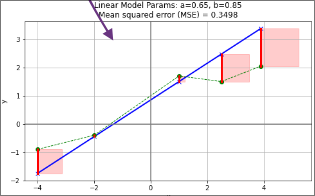
\includegraphics[scale=0.4]{2022-11-04-01:38:51.png}\\
\hline
Annealed SGD & 
\textcolor{orange}{The obvious consequence of this method is that \textbf{the learning effect decays over time,}}\textcolor{red}{this is called \textbf{annealing}.}\newline
\textcolor{orange}{With different options we can control how this curve will drop down. The parameter that we use to represent this curve is called \textbf{alpha}.}\newline
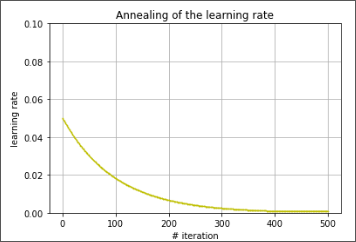
\includegraphics[scale=0.4]{2022-11-04-01:43:27.png}\\
\hline
Limitations & 
\textcolor{purple}{The limitations of this method is that you only use 1 datum -> 1 batch of datapoints for each model. This means that you will have to calculate this over, and over, and over again.\newline
\textbf{In the industry this is usually done in batches of size 32,64,128!}}\newline
\textcolor{orange}{Also, in order to use the SGD the loss function needs to be a \textbf{differentiable function}, this simply means that you can take the derivative of this function at \textbf{every point}. }\newline
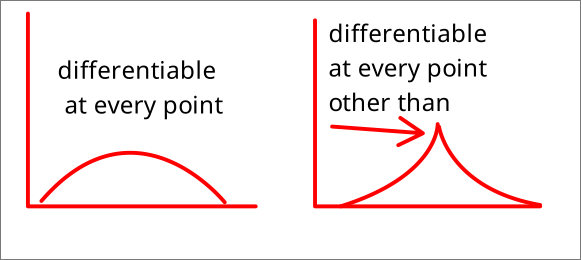
\includegraphics[scale=0.4]{2022-11-04-01:56:28.png}\newline
\textcolor{orange}{On the right side there is the top point where you have 2 interpretations of a derivation, this of course can't be done, so here you would need to define the point manually, or simply use a different function in the first place.}\\
\hline
\end{tabular}
\end{table}
\end{document}
